\documentclass{article}
\usepackage{spikey}
\usepackage{amsmath}
\usepackage{mathrsfs}
\usepackage{amssymb}
\usepackage{soul}
\usepackage{float}
\usepackage{graphicx}
\usepackage{hyperref}
\usepackage{fancyhdr}
\usepackage{xcolor}
\usepackage{chngcntr}
\usepackage{centernot}
\usepackage[shortlabels]{enumitem}
\usepackage[margin=1truein]{geometry}
\usepackage{tkz-graph}
\usepackage{dsfont}
\usepackage{caption}
\usepackage{subcaption}
\usepackage{booktabs}
\usepackage[yyyymmdd,hhmmss]{datetime}

\usepackage{tikz}
\usetikzlibrary{arrows}

\usepackage{setspace}
\linespread{1.15}
\usepackage[margin=1truein]{geometry}

\counterwithin{equation}{section}
\counterwithin{figure}{section}

\usepackage{listings}
 
\definecolor{codegreen}{rgb}{0,0.6,0}
\definecolor{codegray}{rgb}{0.5,0.5,0.5}
\definecolor{codeblue}{rgb}{0.3,0.5,0.8}
\definecolor{codepurple}{rgb}{0.58,0,0.82}
%\definecolor{backcolour}{rgb}{0.95,0.95,0.92}
\definecolor{backcolour}{rgb}{1,1,1}

\lstdefinestyle{mystyle}{
    backgroundcolor=\color{backcolour},   
    commentstyle=\color{codegreen},
    keywordstyle=\color{magenta},
    numberstyle=\tiny\color{codegray},
    stringstyle=\color{codepurple},
    basicstyle=\ttfamily\footnotesize,
    breakatwhitespace=false,         
    breaklines=true,                 
    captionpos=b,                    
    keepspaces=true,                 
    numbers=left,                    
    numbersep=5pt,                  
    showspaces=false,                
    showstringspaces=false,
    showtabs=false,                  
    tabsize=4
}

\lstset{style=mystyle}

\title{CSC413: Homework 3}
\date{\today\ at \currenttime}
\author{Tianyu Du (1003801647)}
\begin{document}
	\maketitle
	\section{Weight Decay}
	\subsection{Under-parameterized Model [0pt]}
	\begin{proof}[Solution]
		Given
	\begin{align}
		\mathcal{J}(\hat{\mathbf{w}})&=\frac{1}{2 n}\|X \hat{\mathbf{w}}-\mathbf{t}\|_{2}^2
		+\frac{\lambda}{2} \hat{\mathbf{w}}^{T} \hat{\mathbf{w}} \\
		\mathcal{J}(\hat{\mathbf{w}})&=\frac{1}{2 n}\|X \hat{\mathbf{w}}-\mathbf{t}\|_{2}^2
		+\frac{\lambda}{2} \norm{\hat{\vew}}_2^2
	\end{align}
	The gradient descent converges when $\frac{d}{d\hat{\vew}} \mathcal{J}(\hat{\mathbf{w}}) = 0$. Altogether with the fact that $\frac{d}{d\vex} \norm{\vex}_2^2 = 2 \vex^T$, the training converges if and only if:
	\begin{align}
		\frac{d}{d\hat{\vew}} \mathcal{J}(\hat{\mathbf{w}})
		&= \frac{1}{n} (X \hat{\vew} - \vet)^T X + \lambda \hat{\vew}^T \\
		&= \frac{1}{n} \hat{\vew}^T X^T X - \frac{1}{n} \vet^T X + \lambda \hat{\vew}^T = 0\quad (\dagger)
	\end{align}
	Note that when $d \leq n$, $rank(X) = d$ implies $X^T X$ is invertible. Suppose $X^T X + n \lambda I$ is invertible as well. Therefore,
	\begin{align}
		(\dagger) &\implies \left(\hat{\vew}^T X^T X + n \lambda \hat{\vew}^T \right) = \vet^T X \\
		&\implies \hat{\vew}^T \left(X^T X + n \lambda I \right) = \vet^T X \\
		&\implies \hat{\vew}^T = \vet^T X \left(X^T X + n \lambda I \right)^{-1} \\
		&\implies \hat{\vew} = \left(X^T X + n \lambda I \right)^{-1} X^T \vet
	\end{align}
	\end{proof}
	
	\subsection{Over-parameterized Model}
	\subsubsection{Warmup: Visualizing Weight Decay [1pt]}
	\begin{proof}[Solution]
		Given 
		\begin{align}
			\vex_1 = (2, 1)\tx{ and } t_1 = 2.
		\end{align}
		From previous homework, the solution of gradient descent without regularization is
		\begin{align}
			\vew^* = \left(\frac{4}{5}, \frac{2}{5} \right)
		\end{align}
		From the previous part, the gradient descent converges if and only if
		\begin{align}
			\frac{d}{d\hat{\vew}} \mathcal{J}(\hat{\mathbf{w}})
			&= \frac{1}{n} (X \hat{\vew} - \vet)^T X + \lambda \hat{\vew}^T \\
			&= ((2,1)\cdot (w_1, w_2) - 2) (2, 1) + \lambda (w_1, w_2) \\
			&= (2 w_1 + w_2 - 2) (2, 1) + (\lambda w_1, \lambda w_2) = 0 \\
		\end{align}
		Therefore, the solution to gradient descent with weight decay is:
		\begin{align}
			&\begin{cases}
				4 w_1 + 2 w_2 -4 + \lambda w_1 &= 0 \\
				2 w_1 + w_2 - 2 + \lambda w_2 &= 0
			\end{cases} \\
			\implies &\begin{cases}
				w_1^* &= \frac{4}{\lambda +5} \\
				w_2^* &= \frac{2}{\lambda +5}
			\end{cases}
		\end{align}
		The solution space is parameterized by $\lambda$ as following
		\begin{align}
			\mc{S} := \left \{
			\frac{4}{\lambda +5}, \frac{2}{\lambda +5}: \lambda \in \R_+
			\right \}
		\end{align}
		which is a singleton uniquely determined by $\lambda$. Note that the following visualization assumes $\lambda = 1$.
		\begin{figure}[H]
			\centering
			\small
			\caption{Visualization}
			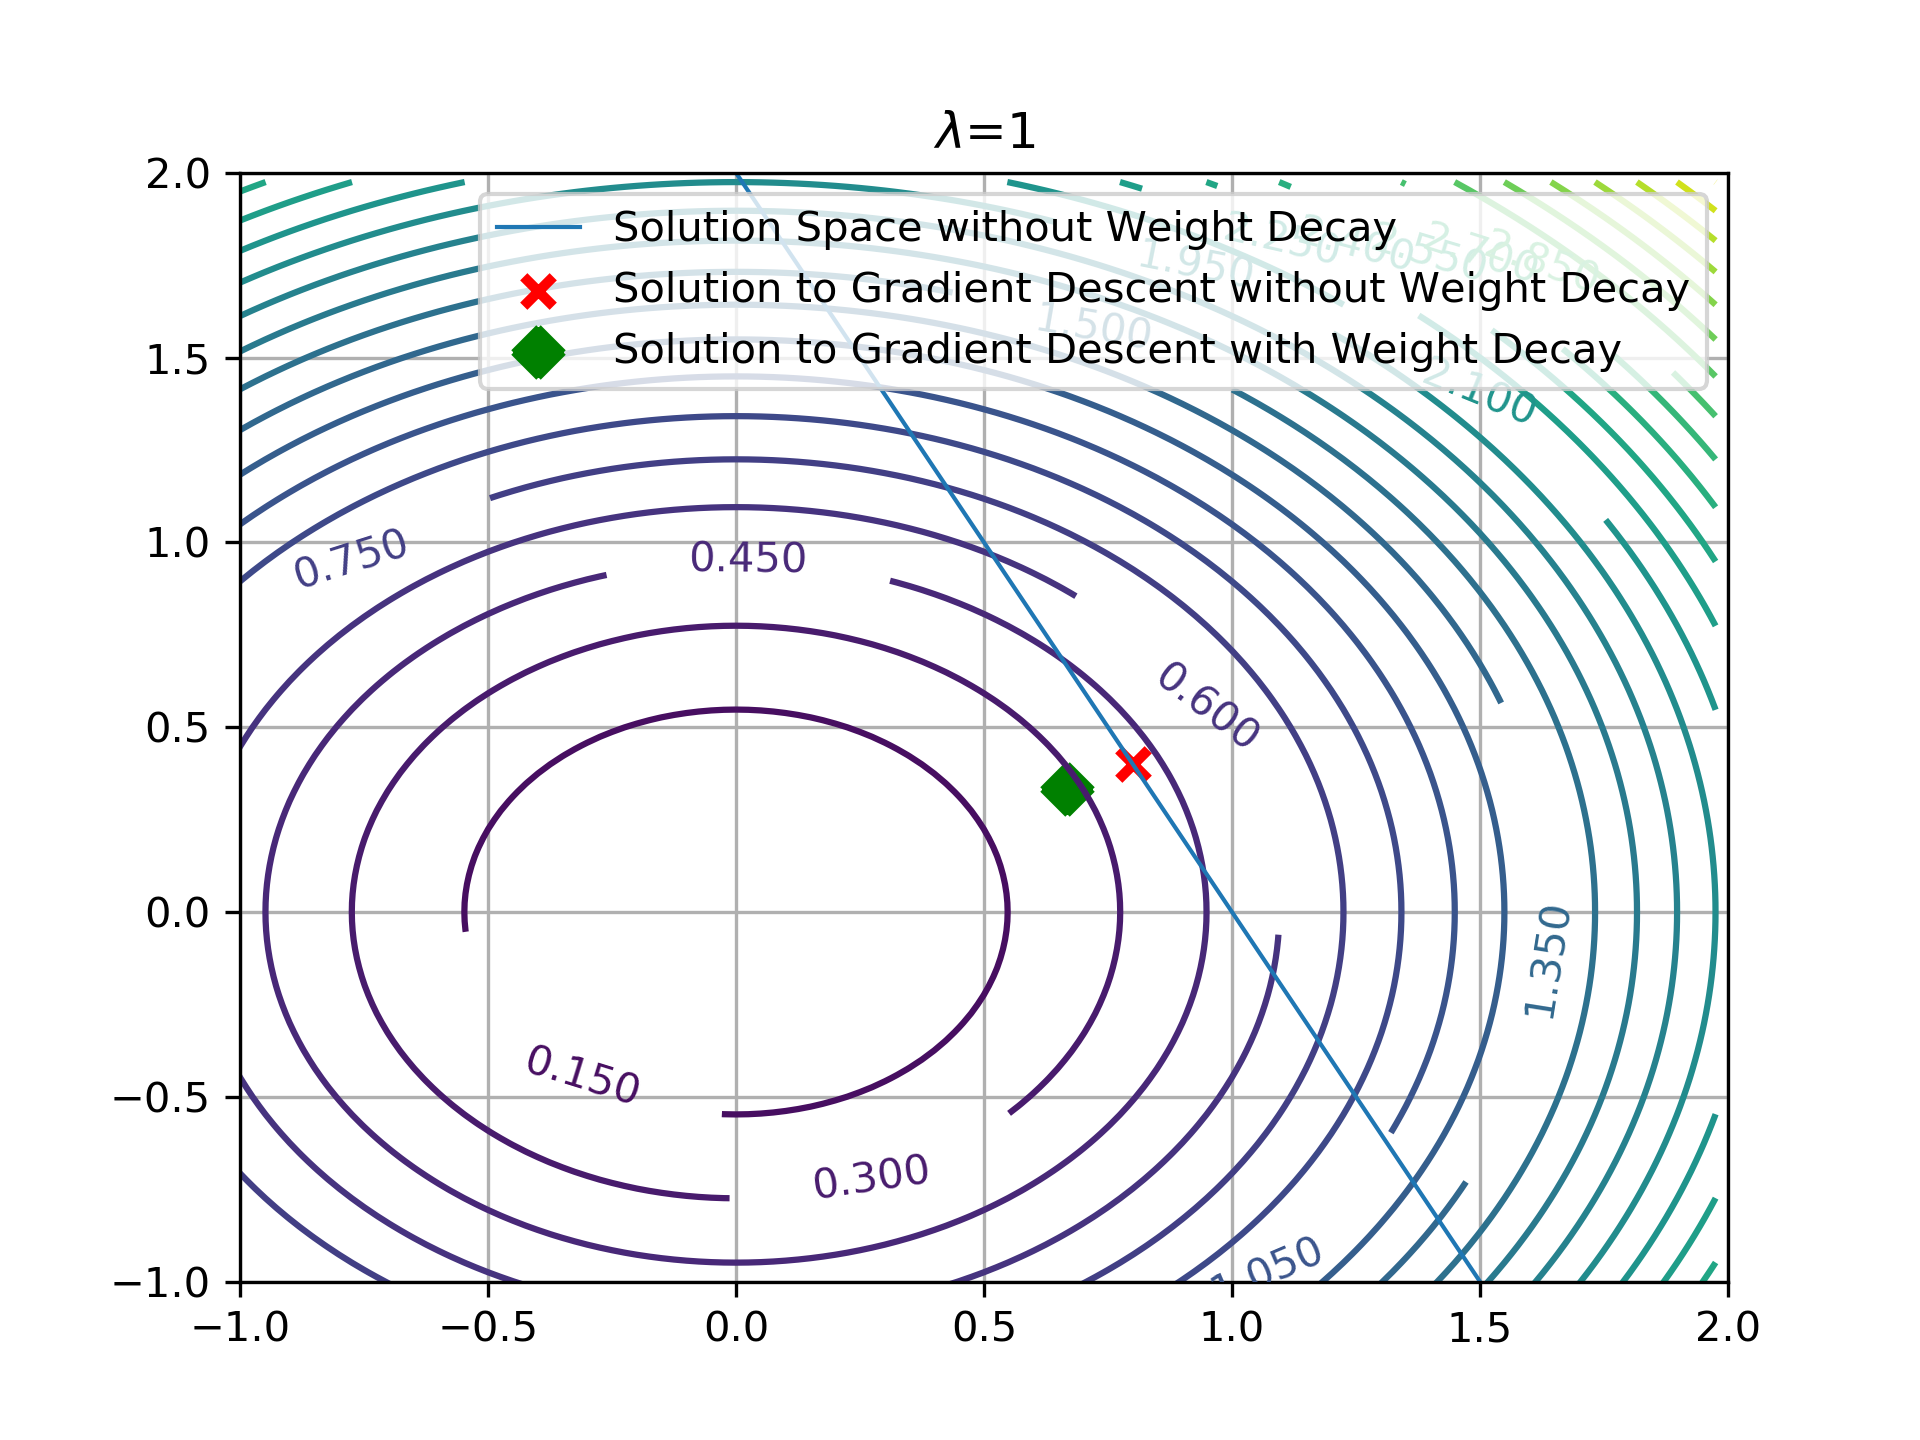
\includegraphics[width=\linewidth]{plot_q1.png}
		\end{figure}
	\end{proof}
	
	\subsubsection{Gradient Descent and Weight Decay [0pt]}
	\begin{proof}[Solution]
		The solution to gradient descent with weight decay has been derived in the previous section:
		\begin{align}
			\vew^*_\tx{weight decay} = \left(\frac{4}{\lambda +5}, \frac{2}{\lambda +5}\right)
		\end{align}
	\end{proof}
	
	\subsection{Adaptive optimizer and Weight Decay [1pt]}
	
	\section{Ensembles and Bias-variance Decomposition}
	\subsection{Weight Average or Prediction Average?}
	\subsubsection{[1pt]}
	\begin{proof}[Solution]
		Without loss of generality, assume the bias is zero. This is equivalent to inserting a column of ones to the $X$, so that $X \in \R^{n \times (d+1)}$, and we can ignore the bias.
	\end{proof}
	
	\section{Generalization and Dropout}
	\subsection{Regression Coefficients}
	\subsubsection{Regression from $X_1$ [0pt]}
	\begin{proof}[Solution]
		
	\end{proof}
	
	\subsubsection{Regression from $X_2$ [1pt]}
	\begin{proof}[Solution]
		Since we are using $X_2$ only, equivalently, we can set the weight of $X_1$ to zero:
		\begin{align}
			\mc{J} &= \expe_{(x_2, y) \sim (X_2, Y)} [(y - \hat{y})^2] \\
			&= \expe_{(x_2, y) \sim (X_2, Y)} [(y - w_2 x_2)^2] \\
			&= \expe_{(x_2, y) \sim (X_2, Y)} [(y - w_2 (y + Gaussian(0, 1)))^2] \\
			&= \expe_{(x_2, y) \sim (X_2, Y)} [((1 - w_2)y - w_2 Gaussian(0, 1) )^2] \\
			&= \expe_{(x_2, y) \sim (X_2, Y)} [((1 - w_2)y)^2] + w_2^2 \expe_{(x_2, y) \sim (X_2, Y)}[Gaussian(0, 1)^2] \\
			&= (1 - w_2)^2 \expe_{y \sim Y} [y^2] + w_2^2
		\end{align}
		Taking the gradient and solve the first order condition:
		\begin{align}
			&\nabla_{w_2} (1 - w_2)^2 \expe_{y \sim Y} [y^2] + w_2^2 = 0 \\
			&\implies - 2(1 - w_2) \expe_{y \sim Y} [y^2] + 2 w_2 = 0 \\
			&\implies \expe_{y \sim Y} [y^2] - w_2 \expe_{y \sim Y} [y^2] - w_2 = 0 \\
			&\implies \expe_{y \sim Y} [y^2] + w_2 (1- \expe_{y \sim Y} [y^2]) = 0 \\
			&\implies w_2 = \frac{\expe_{y \sim Y} [y^2]}{\expe_{y \sim Y} [y^2] + 1}
		\end{align}
		The expectation of $y^2$ is
		\begin{align}
			\expe_{y \sim Y} [y^2] &= \expe_{x_1 \sim X_1} (x_1 + Gaussian(0, \sigma^2))^2 \\
			&= 2 \sigma^2 \\
			\implies w_2 &= \frac{2 \sigma^2}{2 \sigma^2 + 1}
		\end{align}
	\end{proof}
	
	\subsubsection{Regression from $(X_1, X_2)$ [1pt]}
	
	\section{Hard-Coding Recurrent Neural Networks [1pt]}
	\begin{proof}[Solution]
		Let $\sigma = \frac{1}{1 + \exp(-z)}$, and $\vex_t = (x_1^t, x_2^t)$ denotes the input feature at time $t$.
		Consider the following recurrent network:
		\begin{align}
			\hat{y}_t &= \sigma(\vew_{hy} \veh_t + b_y)\\
			\veh_t &= \sigma(\vew_{hh} \veh_{t-1} + \vew_{xh} \vex_t + b_h)
		\end{align}
		with the following parameters:
		\begin{align}
			\vew_{xh} &= 
			\begin{pmatrix}
				a & b \\ c & d
			\end{pmatrix}
			\\
			\vew_{hh} &= 
			\begin{pmatrix}
				a & b \\ c & d
			\end{pmatrix}
			\\
			b_h &= 0
			\\
			\vew_{hy} &= 
			\begin{pmatrix}
				a & b \\ c & d
			\end{pmatrix}
			\\
			b_y &= 0
		\end{align}
		\emph{Justification:} \\
	\end{proof}
\end{document}






























